\documentclass{article}

\usepackage[T1]{fontenc}
\usepackage[utf8]{inputenc}
\usepackage{times}
\usepackage[margin=1in]{geometry}
\usepackage{natbib}
\usepackage{amsmath}
\usepackage{amssymb}
\usepackage{booktabs}
\usepackage{microtype}
\usepackage{tabularx}
\newcolumntype{Y}{>{\raggedright\arraybackslash}X}
\usepackage{tikz}
\usepackage{pgfplots}
\usepackage{float}
\usepackage{url}
\usepackage{hyperref}
\hypersetup{
  hidelinks,
  pdftitle={LeanNumBench: Diagnosing LLM Proof Completion in Lean-Checked Numerical Analysis},
  pdfauthor={Qinghe Wang}
}
\usetikzlibrary{arrows.meta,positioning}
\pgfplotsset{compat=1.18}


\title{LeanNumBench: Diagnosing LLM Proof Completion in Lean-Checked Numerical Analysis}

\author{Qinghe Wang\\
Independent Researcher}

\date{June 2026}

\begin{document}

\maketitle

\begin{abstract}
Language models increasingly solve Lean theorem-proving tasks, but aggregate
pass rates can hide whether they can compose the local proof-engineering
patterns needed in verified scientific computing. We introduce LeanNumBench,
a Lean 4 diagnostic benchmark for numerical-analysis proof-body completion.
LeanNumBench v1 contains 160 frozen proof-completion records spanning finite
differences, FEM/P0 projection, spectral identities, ODE and Runge--Kutta
identities, linear-algebra stability, interpolation, and quadrature. Each
record exposes a Lean theorem statement together with fixed local declarations,
and model outputs are checked locally without accepting \texttt{sorry}. In a
dated May-2026 five-endpoint panel, the strongest pre-specified endpoint
solves 147/160 records, but 11 records are failed by at least three endpoints.
A hard-row pass@3 probe, declaration-context ablation, repair audit, and
failure taxonomy show that residual failures are primarily proof-search and
tactic-composition failures, rather than missing-identifier failures. The
benchmark therefore turns routine-looking numerical-analysis lemmas into an
auditable diagnostic for where direct Lean proof completion still breaks.
\end{abstract}

\section{Introduction}

Formal theorem proving has become a central testbed for evaluating language
models as mathematical assistants. Lean 4 offers a strict evaluation setting:
a candidate proof either elaborates against the local environment or it does
not. That strictness is useful, but it also makes benchmark design delicate.
If a benchmark only reports a flat pass rate, it can miss the proof-engineering
surface that determines whether models are useful in a scientific domain.

Numerical analysis is a useful stress test because many of its formalization
tasks are local, structured, and computational rather than long
Olympiad-style searches. Finite sums telescope; boundary terms cancel; CFL
conditions make update weights nonnegative; projection residuals are
orthogonal; finite Fourier means normalize; row-stochastic operators preserve
$L_\infty$ bounds. Informally, these facts can look routine. In Lean, they
often require exact control of local definitions, helper lemmas, normalization
steps, order side conditions, and APIs such as \texttt{Finset}, absolute
values, \texttt{max\_le}, \texttt{mul\_le\_mul}, and arithmetic tactics. A
model that recognizes the mathematics can still fail to compose a
Lean-checking proof.

Current formal-proving benchmarks have made rapid progress, but they emphasize
different evaluation surfaces. Contest-style and undergraduate benchmarks
stress standalone mathematical problem solving; large Lean benchmarks stress
scale, retrieval, or broad domain coverage; applied-mathematics benchmarks
stress either broad computational coverage or construction-verification
workflows. LeanNumBench isolates a narrower surface: proof-body completion for
numerical-analysis lemmas under frozen local declaration context. This setting
is close to the day-to-day proof-engineering bottleneck in verified scientific
computing: the model is not asked to discover a theorem statement or construct
a global proof-search strategy, but to compose a Lean-checking local proof from
available definitions, helper lemmas, and Mathlib APIs. It deliberately trades
breadth for record-level provenance, frozen local context, Lean-checked proof
bodies, hard-subset analysis, ablations, and a failure taxonomy. It is not
intended to be the broadest applied-math benchmark, a complete numerical-analysis
library, or an agentic proof-search environment. It asks a narrower question:
when dated model endpoints receive a theorem statement and relevant local Lean
context, which numerical-analysis proof patterns still break, and why?

\begin{table}[H]
\centering
\caption{LeanNumBench is intended as a diagnostic complement to broader Lean applied-mathematics benchmarks.}
\label{tab:benchmark-positioning}
\scriptsize
\begin{tabularx}{\linewidth}{lYYY}
\toprule
Axis & CAM-Bench & AMBER / Construction-Verification & LeanNumBench\\
\midrule
Primary task & Broad applied-math Lean targets & Construct-and-verify tasks
& Proof-body completion\\
Input surface & Theorem/problem target & Construction specification plus
verification & Theorem statement plus frozen local declarations\\
Main unit of evidence & Broad target coverage & Construction-verification
success & Lean-checked model candidate plus row-level diagnostics\\
Artifact emphasis & Benchmark suite & Construction tasks & Prompt packs,
checked candidates, checker logs, repair audit, failure taxonomy\\
Role & Coverage benchmark & Construction stress test & Local proof-failure
diagnostic\\
\bottomrule
\end{tabularx}
\end{table}

The answer is more structured than a leaderboard suggests. Our experiments
give three findings. First, proof completion is still not saturated: in our
May-2026 frozen panel, all five dated endpoint aliases solve most of the
160-record proof set, with accuracies from 78.8\% to 91.9\%, yet 11 rows are
failed by at least three models. A final pass@3 probe improves coverage but
shows persistent per-endpoint fragility rather than absolute unsolvability:
the best endpoint solves 9/11, four rows remain unsolved by at least two
endpoints, and a cross-endpoint oracle solves all 11. Second, local Lean context matters:
a two-model declaration-context ablation changes full-context performance
from 48/74 to 59/74 paired model-row passes.
Third, the residual failures are proof-engineering failures rather than
simple retrieval failures. Our taxonomy shows that 55 of 102 failures are
proof-search or tactic-composition failures, while only 2 are missing-context
or missing-identifier failures.

This paper contributes:

\begin{itemize}
\item \textbf{Dataset.} LeanNumBench v1, a Lean-checked numerical-analysis
proof-completion benchmark with 160 frozen records, 12 theorem-family
categories, provenance metadata, and fixed local declaration context.
\item \textbf{Evaluation harness.} A local checker that materializes model
outputs into Lean candidates and separately reports raw passes,
repair-assisted passes, extraction failures, \texttt{sorry} usage, and Lean
failures.
\item \textbf{Frozen endpoint panel.} A dated May-2026 five-endpoint evaluation
over all 160 proof-completion records, reported as a snapshot rather than a
timeless model ranking.
\item \textbf{Diagnostics.} Hard-subset analysis, pass@3 probing,
declaration-context ablation, deterministic-repair audit, and failure taxonomy.
\item \textbf{Artifact.} Released prompt packs, usage-stripped model outputs,
materialized candidates, checker summaries, table data, and no-API replay
scripts.
\end{itemize}

\begin{figure}[t]
\centering
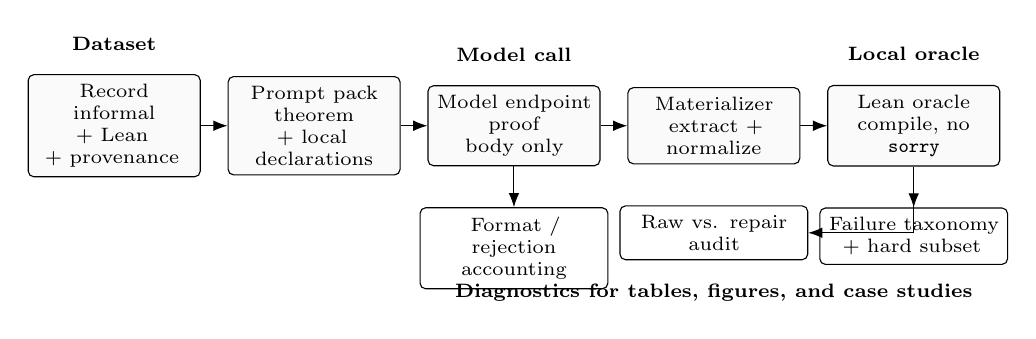
\begin{tikzpicture}[
  node distance=0.52cm and 0.34cm,
  stage/.style={draw, rounded corners=2pt, align=center, minimum height=0.75cm,
                text width=1.95cm, font=\scriptsize, fill=black!2},
  result/.style={draw, rounded corners=2pt, align=center, minimum height=0.65cm,
                 text width=2.15cm, font=\scriptsize},
  label/.style={font=\scriptsize\bfseries, align=center},
  arrow/.style={-{Latex[length=1.8mm]}, line width=0.35pt}
]
\node[stage] (record) {Record\\informal + Lean\\+ provenance};
\node[stage, right=of record] (prompt) {Prompt pack\\theorem + local\\declarations};
\node[stage, right=of prompt] (model) {Model endpoint\\proof body only};
\node[stage, right=of model] (mat) {Materializer\\extract +\\normalize};
\node[stage, right=of mat] (lean) {Lean oracle\\compile, no\\\texttt{sorry}};

\node[result, below=of model] (format) {Format / rejection\\accounting};
\node[result, below=of mat] (repair) {Raw vs. repair\\audit};
\node[result, below=of lean] (tax) {Failure taxonomy\\+ hard subset};

\node[label, above=0.18cm of record] {Dataset};
\node[label, above=0.18cm of model] {Model call};
\node[label, above=0.18cm of lean] {Local oracle};
\node[label, below=0.18cm of repair] {Diagnostics for tables, figures, and case studies};

\draw[arrow] (record) -- (prompt);
\draw[arrow] (prompt) -- (model);
\draw[arrow] (model) -- (mat);
\draw[arrow] (mat) -- (lean);
\draw[arrow] (model) -- (format);
\draw[arrow] (lean) |- (repair);
\draw[arrow] (lean) -- (tax);
\end{tikzpicture}
\caption{LeanNumBench evaluates numerical-analysis proof completion with a
local-first pipeline. Curated records produce prompt packs; model outputs are
materialized into Lean candidates; the local Lean oracle accepts only compiling
proofs without \texttt{sorry}; and the same run emits rejection accounting,
repair auditing, failure taxonomy, and hard-subset case studies.}
\label{fig:leannumbench-pipeline}
\end{figure}


\section{Benchmark Design}

\subsection{Records}

Each LeanNumBench record packages one numerical-analysis theorem with metadata and
tasks. A record contains an informal statement, a LaTeX-style statement, a
Lean theorem declaration, local declarations used by the theorem, source and
provenance metadata, difficulty tags, and the verification target. The
record is not simply a theorem string: it is designed to preserve the
mathematical intent, the Lean environment, and the evaluation task surface.

LeanNumBench v1 contains 160 frozen records and 405 task specifications:
160 proof-completion tasks, 160 statement-translation tasks, and 85
theorem-retrieval tasks. The proof-completion task is the primary evaluation
setting in this paper; statement translation is used only as a calibration
slice, and theorem retrieval is included in the artifact but not evaluated as a
headline result. The model receives the theorem statement and local declaration
context, then must output only the proof body after \texttt{:= by}. Candidate
outputs are checked locally against the companion Lean project; \texttt{sorry}
is not accepted as a proof.

\subsection{Mathematical Scope}

LeanNumBench focuses on numerical-analysis theorem shapes rather than broad
coverage of all applied mathematics. The 160-record v1 release spans 12
families (Table~\ref{tab:families}). The goal is not to maximize theorem
count. For a diagnostic benchmark, the unit of evidence is the checked
record--model interaction plus controlled analysis around it: the final panel
contains 800 model-record attempts, 786 materialized Lean candidates, and
targeted pass@3, context, repair, provenance, and failure analyses. The dataset is curated to expose recurring
proof surfaces: finite sums and telescoping, boundary bookkeeping, CFL
convexity, local definition unfolding, operator/norm inequalities, projection
orthogonality, spectral normalization, and elementary interpolation or
quadrature algebra. Short rows are useful when they isolate a Lean
proof-engineering failure that is easy to miss in aggregate metrics.

\begin{table}[H]
\centering
\caption{Family coverage in the 160-record LeanNumBench v1 release.}
\label{tab:families}
\small
\begin{tabular}{lr}
\toprule
Family & Records\\
\midrule
FEM/P0 projection & 28\\
finite-difference KdV & 25\\
spectral/DFT identities & 23\\
finite-difference heat & 15\\
linear-algebra stability & 14\\
finite-difference Burgers & 10\\
finite-difference stability & 10\\
finite-difference conservation & 8\\
interpolation & 8\\
ODE symplectic invariants & 7\\
Runge--Kutta identities & 6\\
quadrature & 6\\
\bottomrule
\end{tabular}
\end{table}

\subsection{Provenance}

LeanNumBench v1 includes 59 records with textbook or paper provenance, 4
classic/general records, and 97 internal Lean-seed records. Provenance is used
to document mathematical motivation and reduce the risk that the dataset is a
purely self-invented Lean exercise set. The Lean ground truth remains the
companion formalization, while the provenance records the mathematical family
and source alignment. LeanNumBench is not automatically mined from external
corpora, and we do not claim that each record is a verbatim formalization of a
textbook theorem. This is a curated diagnostic benchmark: provenance supports
interpretability and audit, but the evaluation object is the Lean-checked
proof task. In the final five-endpoint panel, textbook/paper records account for
295 model-record pairs with 253 passes (85.8\%), while internal Lean-seed
records account for 485 pairs with 430 passes (88.7\%); both strata therefore
contribute to the measured signal.

\subsection{Dataset Construction And Leakage Audit}

The benchmark is frozen before the reported model panel. A record enters the
release only after the theorem statement elaborates, the ground-truth proof is
complete in the companion Lean project, and the prompt audit confirms target
and local-declaration alignment. The May-2026 freeze note records 160 records,
405 task specifications, a 14/14 local smoke-check pass, and a zero-issue
160-row proof-prompt audit. The audit checks that prompt, target, and candidate
template rows are aligned; candidate templates are empty; target proof hints
are not copied verbatim into prompts; and the pre-target source-context block
does not include the target theorem header.

The 160-record release covers 160 of 176 companion theorem declarations. The
remaining 16 are tracked as a future-expansion backlog rather than used as a
hidden split: 10 are simple shape-balancing candidates in interpolation,
quadrature, and symplectic one-step maps, while 6 are mostly additional
conservation/KdV wrappers. Prompt audits check for author-identifying paths
and repository-owner strings, and the released artifact strips raw usage
metadata from model-output logs. The proof task exposes the theorem statement
and local declarations by design: LeanNumBench is not a memorization-free
theorem-retrieval benchmark, but a Lean-checked proof-body completion benchmark
under fixed local context. The leakage claim is therefore narrow: the audit
rules out copied target hints, target-theorem duplication in the local context,
nonempty candidate templates, and environment-specific contamination, not
semantic independence from all nearby helper lemmas.

\section{Evaluation Pipeline}

Figure~\ref{fig:leannumbench-pipeline} summarizes the evaluation pipeline. Records
are converted into prompt packs; model outputs are assembled into Lean proof
candidates; and the Lean checker verifies each candidate against the companion
formalization. The output is not only pass/fail. The pipeline records
extraction failures, empty proof bodies, deterministic repair steps, Lean
error categories, \texttt{sorry} usage, and hard-subset membership.

The materialization stage is important because model outputs often contain
Markdown fences, repeated theorem statements, explanatory text, or accidental
indentation. LeanNumBench separates these pipeline outcomes from Lean failures.
This avoids silently converting formatting errors into proof failures or
silently accepting non-proof text.

The checker supports a narrow deterministic repair mode. It may drop a tactic
line that Lean reports made no progress, replace a failing \texttt{ring} with
\texttt{ring\_nf} when Lean suggests that shape, or drop a redundant final
tactic when Lean reports no goals remain. It does not synthesize new
mathematical proof steps, call an LLM, or search for new lemmas. We report
repair-assisted passes separately from raw passes.

We freeze dated endpoint protocols rather than claiming timeless rankings. Model
APIs change quickly, and a benchmark paper should not pretend that a
May-2026 endpoint table is a permanent ordering. LeanNumBench therefore uses
dated prompt packs, explicit endpoint aliases, small rolling probes for new
endpoints, and a final frozen panel only when the dataset and manuscript are
stable.

\section{Dataset Verification And Artifact Policy}

The 160-record v1 release passes schema validation and Lean smoke
checking. The smoke suite contains 14 verification suites and passes all 14.
The frozen 160-record proof prompt pack has a zero-issue prompt audit: each
prompt, target theorem, and generated proof obligation is aligned. A separate
artifact audit checks that released prompts do not expose author identity or
environment-specific paths.
The companion artifact contains the frozen records, prompt packs,
companion Lean source, API-free replay model-output logs, generated
tables, and offline audit scripts. Reproduction does not require model API
calls: readers can rerun metadata and identity/path checks directly, and can
rerun Lean checking locally after fetching the public Mathlib dependencies
specified by the included Lake files. The released companion Lean tree is
audited for benchmark-relevant placeholders: this release contains no
\texttt{sorry}, \texttt{admit}, or user-defined \texttt{axiom} declarations.
Its Lean toolchain is \texttt{leanprover/lean4:v4.29.1}, the Mathlib
dependency is pinned to revision \texttt{v4.29.1}, and the corresponding Lake
files are included with the released companion Lean project.

\section{Experiments}

The experiments are designed as diagnostics rather than a model race. We ask
six questions. First, can a fixed tactic portfolio solve the benchmark without
model generation? Second, is numerical-analysis proof completion already
saturated by dated endpoint aliases? Third, is proof completion more
discriminating than statement translation on a calibration slice? Fourth, do
the remaining failures persist for individual endpoints under sampling, or are
they one unlucky decoding? Fifth, does local Lean declaration context
materially affect success? Sixth, are the reported passes driven by
deterministic repair? Section~\ref{sec:failure-taxonomy} then asks what kind
of failures remain after materialization and local checking.

\subsection{Fixed Tactics Do Not Saturate LeanNumBench}

As a no-LLM sanity baseline, we run a fixed portfolio of 13 generic Lean tactic
scripts over all 160 v1 proof-completion statements, including reflexivity,
simplification, arithmetic normalization, linear/nonlinear arithmetic, and
\texttt{aesop}. The portfolio solves 68/160 records (42.5\%); individual
tactics solve at most 59/160 (36.9\%). Thus the high endpoint scores
below are not explained by the benchmark collapsing to one-step automated
tactics.

\subsection{Proof Completion Is High But Not Saturated}

We evaluate five dated third-party endpoint aliases on the May-2026
160-record frozen proof-completion panel. Candidates are checked locally and
reported only when they pass without \texttt{sorry}. We report these as
endpoint results, not immutable model-version results.

\begin{table}[H]
\centering
\caption{May-2026 proof-completion panel over all 160 LeanNumBench v1 records.}
\label{tab:proof-snapshot}
\small
\begin{tabular}{lrr}
\toprule
Endpoint alias & Passed & Accuracy\\
\midrule
Gemini 3.1 Pro Preview & 147/160 & 91.9\%\\
GPT-5.5 Pro & 145/160 & 90.6\%\\
Claude Opus 4.8 & 141/160 & 88.1\%\\
Qwen3.6 Max Preview & 139/160 & 86.9\%\\
DeepSeek v4 Pro & 126/160 & 78.8\%\\
\bottomrule
\end{tabular}
\end{table}

Table~\ref{tab:proof-snapshot} shows high aggregate accuracy with persistent
row-level failures. The top endpoint in this pre-specified five-endpoint panel
scores 147/160, and the five-endpoint spread is 13.1 percentage points, but
Wilson 95\% intervals overlap for the top rows (86.6--95.2\% for 147/160 and
85.1--94.2\% for 145/160). We therefore do not treat this dated panel as a
stable model ranking. Its role is to expose which proof patterns remain
unsolved after high aggregate performance. Additional post-freeze
endpoint-variant probes are reported in the appendix only as evidence of
endpoint churn; they are not used to define the main panel, hard subset, or
failure taxonomy.

\subsection{Proof Completion Is More Discriminating Than Statements}

We also evaluate a dated 50-record statement-translation snapshot. Statement
translation is nearly saturated in this snapshot: Claude Opus 4.7,
DeepSeek v4 Pro, and GPT-5.5 Pro solve 50/50 checked statement candidates;
Gemini 3.1 Pro Preview and Qwen3.6 Max Preview solve 49/50. This contrast is
useful because it rules out a weaker interpretation of the benchmark: the
main difficulty is not simply writing Lean theorem headers that elaborate on
this calibration slice. We do not treat the 50-record statement run as a full
secondary leaderboard. Its role is to support the qualitative comparison:
once the formal statement is fixed, proof completion remains the more
discriminating task in our evidence.

\subsection{Hard Rows Persist In The Frozen Panel}

We define a hard subset as rows failed by at least three of five models in the
one-shot 160-record frozen panel. This yields 11 rows covering FEM/P0
projection, finite-difference stability, KdV definition unfolding, heat/CFL
side conditions, spectral centered-DC normalization, and linear-algebra norm
bounds.

Five of the 11 hard rows are failed by four of five endpoints, and six are
failed by three of five endpoints. We then run a final five-endpoint pass@3
probe over the 11 hard rows. This post-hoc probe is a robustness check on
persistent rows, not an unbiased estimate of pass@3 over the full benchmark.
Sampling improves coverage: every hard row is solved by at least one endpoint
under pass@3. Thus the claim is not absolute unsolvability: a cross-endpoint
oracle would solve all 11. The diagnostic signal is per-endpoint fragility.
The best endpoints solve 9/11 rows, and four rows remain unsolved by at least
two of five endpoints.

\begin{table}[H]
\centering
\caption{Representative hard rows remain diagnostic under pass@3.}
\label{tab:hard-subset-mini}
\scriptsize
\begin{tabularx}{\linewidth}{Xrrr}
\toprule
Hard row & One-shot failures & Models solved by pass@3 & Passing samples\\
\midrule
P0 projection idempotence & 4/5 & 2/5 & 6/15\\
Weighted P0 residual mass zero & 4/5 & 3/5 & 5/15\\
KdV canonical flux const-difference & 3/5 & 2/5 & 4/15\\
Diagonal infinity-norm bound & 3/5 & 1/5 & 3/15\\
\bottomrule
\end{tabularx}
\end{table}

\subsection{Local Declaration Context Is Part Of The Task}

To test whether local Lean declarations matter, we construct a paired 37-row
ablation. The full-context prompt includes local declaration names available
through imports. The no-declaration-context prompt removes that block while
preserving the theorem statement, record-local definitions listed in metadata,
proof-output rules, and domain-specific guidance. This is not a no-hint
ablation; it isolates the declaration-context block.

For DeepSeek v4 Pro, full declaration context solves 27/37 while no-context
solves 20/37; for Gemini 3.1 Pro Preview, the corresponding numbers are 32/37
and 28/37. Aggregated over the two models, full context solves 59/74
model-row pairs while no-context solves 48/74. Row-level flips remain
non-monotone: full context helps on 16 paired rows, no-context helps on 5,
both pass on 43, and both fail or reject on 10. An exact two-sided sign test
over the 21 discordant model-row pairs gives \(p=0.0266\), but this
descriptive test treats paired rows and model endpoints as independent and
therefore ignores row/model clustering. We read it as exploratory evidence,
not a confirmatory population-level claim. Thus LeanNumBench measures
context-sensitive proof engineering, not just isolated mathematical recall. An
appendix 8-pair controlled proof-surface pilot gives the same qualitative
signal: in aggregate, two independent model families solve exposed proof
surfaces more often than matched harder surfaces, but the pilot is diagnostic
rather than a headline benchmark result.

\subsection{Simple Repair Does Not Explain The Leaderboard}

The evaluation pipeline uses a narrow deterministic repair mode, and we report
its effect separately from raw checking. On the 73-record delta slice across
five models, simple repair changes 306 raw passes to 313 final passes, a lift
of 7 pairs or 1.9 percentage points. In the final 160-record panel, only
17/800 model-record attempts are repair-assisted passes (2.1\%, Wilson 95\% CI
1.3--3.4\%). All repair-assisted passes come from dropping redundant no-goals
tactic lines; no reported pass uses \texttt{sorry}. The leaderboard is
therefore not driven by hidden post-processing, and the remaining failures
should be read as proof-generation failures rather than artifacts of a
permissive repair loop.

\begin{figure}[H]
\centering
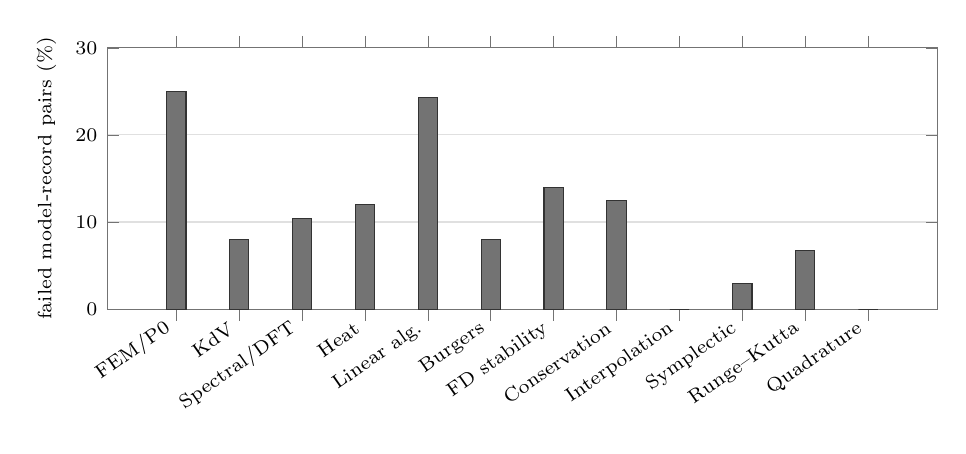
\begin{tikzpicture}
\begin{axis}[
  ybar,
  width=\linewidth,
  height=4.9cm,
  bar width=7pt,
  ymin=0,
  ymax=30,
  ylabel={failed model-record pairs (\%)},
  symbolic x coords={{FEM/P0},{KdV},{Spectral/DFT},{Heat},{Linear alg.},{Burgers},{FD stability},{Conservation},{Interpolation},{Symplectic},{Runge--Kutta},{Quadrature}},
  xtick=data,
  x tick label style={rotate=35, anchor=east, font=\scriptsize},
  tick label style={font=\scriptsize},
  label style={font=\scriptsize},
  ymajorgrids=true,
  grid style={black!12},
  axis line style={black!55},
  tick style={black!55}
]
\addplot+[draw=black!80, fill=black!55] coordinates {
({FEM/P0},25.0)
({KdV},8.0)
({Spectral/DFT},10.4)
({Heat},12.0)
({Linear alg.},24.3)
({Burgers},8.0)
({FD stability},14.0)
({Conservation},12.5)
({Interpolation},0)
({Symplectic},2.9)
({Runge--Kutta},6.7)
({Quadrature},0)
};
\end{axis}
\end{tikzpicture}
\caption{Failure rate by theorem family in the May-2026 5-model proof panel.
Failures concentrate in FEM/P0 projection, linear-algebra stability, FD
stability, conservation, heat/CFL, and spectral/DFT rows rather than uniformly
across families.}
\label{fig:coverage-failure}
\end{figure}

\begin{figure}[H]
\centering
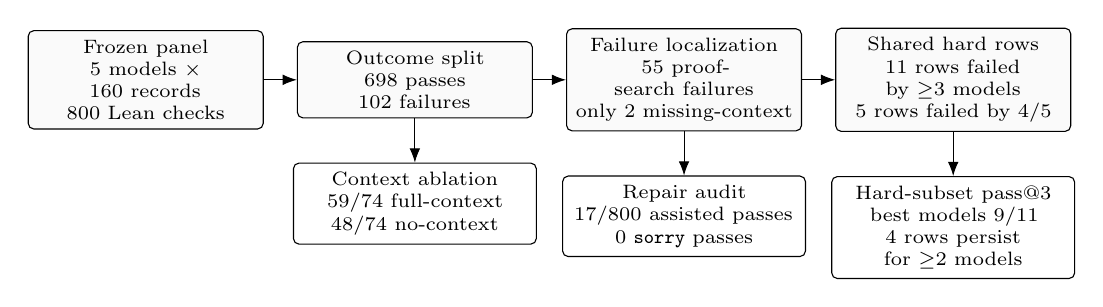
\begin{tikzpicture}[
  node distance=0.42cm and 0.42cm,
  box/.style={draw, rounded corners=2pt, align=center, minimum height=0.82cm,
              text width=2.75cm, font=\scriptsize, fill=black!2},
  smallbox/.style={draw, rounded corners=2pt, align=center, minimum height=0.72cm,
                   text width=2.85cm, font=\scriptsize},
  arrow/.style={-{Latex[length=1.8mm]}, line width=0.35pt}
]
\node[box] (panel) {Frozen panel\\5 models $\times$ 160 records\\800 Lean checks};
\node[box, right=of panel] (split) {Outcome split\\698 passes\\102 failures};
\node[box, right=of split] (tax) {Failure localization\\55 proof-search failures\\only 2 missing-context};
\node[box, right=of tax] (hard) {Shared hard rows\\11 rows failed by $\geq$3 models\\5 rows failed by 4/5};

\node[smallbox, below=0.56cm of split] (context) {Context ablation\\59/74 full-context\\48/74 no-context};
\node[smallbox, below=0.56cm of tax] (repair) {Repair audit\\17/800 assisted passes\\0 \texttt{sorry} passes};
\node[smallbox, below=0.56cm of hard] (passk) {Hard-subset pass@3\\best models 9/11\\4 rows persist for $\geq$2 models};

\draw[arrow] (panel) -- (split);
\draw[arrow] (split) -- (tax);
\draw[arrow] (tax) -- (hard);
\draw[arrow] (split) -- (context);
\draw[arrow] (tax) -- (repair);
\draw[arrow] (hard) -- (passk);
\end{tikzpicture}
\caption{LeanNumBench turns a high aggregate pass rate into a diagnostic object. The
frozen panel first separates passes from Lean-checked failures, then localizes
the dominant residual failure mode, identifies shared hard rows, and probes
whether those rows persist under sampling. Context and repair audits check that
the signal is not merely missing declarations or permissive post-processing.}
\label{fig:diagnostic-panel}
\end{figure}


\section{Failure Taxonomy}
\label{sec:failure-taxonomy}

The failure taxonomy asks a more important question than the leaderboard:
after a model has seen the theorem statement and local declarations, why does
the candidate still fail Lean, or fail before Lean checking? The five-endpoint
by 160-record frozen panel contains 800 model-record attempts
(Figure~\ref{fig:diagnostic-panel}). Of these, 786 materialize as Lean proof
candidates, 698 pass, 88 materialized candidates fail Lean, and 14 attempts
are pre-Lean pipeline failures. These 14 are kept separate from Lean checker
failures: 12 are model-output/materialization failures caused by empty proof
bodies, and 2 are API/transport failures after the fixed collection protocol.
We classify the 102 total non-pass outcomes.
Proof-search or tactic-composition failures account for 55 of 102 non-pass
outcomes (53.9\%, Wilson 95\% CI 44.3--63.3\%). Other Lean failures account
for 14 outcomes, rejected empty proof bodies for 12, type mismatch or
typeclass issues for 9, Lean syntax errors for 8, missing context or missing
identifiers for 2, and API/transport failures for 2.

This is the main diagnostic result. The residual failures are not primarily
unknown names or absent imports. They are unsolved goals, failed rewrites,
arithmetic/inequality tactics that do not close, local algebra left in the
wrong normal form, or malformed proof blocks after partial progress. In other
words, the bottleneck is proof construction under Lean checking, not just
retrieval. The categories are assigned by fixed priority rules described in
the appendix, and the artifact includes row-level model outputs, check
reports, and failure-category summaries for audit.

The family-level distribution supports the same interpretation. The highest
failure rates appear in FEM/P0 projection and linear-algebra stability, with
additional pressure in finite-difference stability, conservation, heat/CFL, and
spectral/DFT rows (Figure~\ref{fig:coverage-failure}). These are exactly the
families where informal numerical analysis hides proof-engineering pressure:
projection algebra, CFL convexity, definition unfolding, finite sums, and norm
inequalities.

\section{Hard-Subset Case Studies}
\label{sec:case-studies}

The final 11-row hard subset makes the aggregate taxonomy concrete.
Table~\ref{tab:representative-residues} shows three recurring failure
mechanisms. The cases below then expand on them.

\begin{table}[H]
\centering
\caption{Representative hard rows and typical failed residues.}
\label{tab:representative-residues}
\scriptsize
\begin{tabularx}{\linewidth}{
  >{\raggedright\arraybackslash}p{0.22\linewidth}
  >{\raggedright\arraybackslash}p{0.25\linewidth}
  >{\raggedright\arraybackslash}p{0.25\linewidth}
  >{\raggedright\arraybackslash}X}
\toprule
Row & Informal math & Lean obstacle & Diagnostic lesson\\
\midrule
Lax--Friedrichs CFL stability & Convex combination preserves
\(L_\infty\) bounds & Absolute values, nonnegative weights, and both
inequality directions must align & Recognizing convexity is not enough for a
Lean-checking inequality proof.\\
Centered DC zero mode & Subtracting the finite mean kills the DC component &
\texttt{Finset} rewriting, constant sums, and nonzero-cardinality algebra &
Finite-sum normalization is a first-class proof-engineering obstacle.\\
P0 projection idempotence & Averaging projected cell values is idempotent &
Local projection API unfolding and normal form & Short numerical-analysis
lemmas can fail on local definition choreography.\\
\bottomrule
\end{tabularx}
\end{table}

\paragraph{Lax--Friedrichs CFL $L_\infty$ stability.}
The Lax--Friedrichs CFL stability row is failed by four of five endpoints in the
final panel. The proof is a small CFL convex-combination argument: use
nonnegative weights, distribute absolute values, combine max bounds, and close
arithmetic. In Lean, this becomes a brittle chain of local lemma selection,
absolute-value rewriting, and inequality side conditions. This row separates
recognizing a textbook stability argument from producing a checker-valid
inequality proof.

\paragraph{Centered signal has zero DC mode.}
The general-$N$ centered-DC row is a finite-sum normalization fact:
subtracting the finite mean makes the DC sum vanish. Several models reach a
nearly algebraic remaining goal but fail to align \texttt{Finset} rewriting,
constant sums, and the nonzero-cardinality assumption. This is a finite-sum
bookkeeping failure, not a failure to understand the mathematical statement.

\paragraph{P0 projection idempotence.}
The two-cell P0 projection-idempotence row is short and mathematically
elementary: averaging projected cell values gives the same average. Yet
multiple models unfold only part of the local projection API or leave Lean
with a normal-form mismatch. This demonstrates why small rows still matter:
numerical-analysis formalization often fails on local definition unfolding and
normalization details that informal mathematics hides. The case studies
therefore justify LeanNumBench's diagnostic design: the hardest rows are not
necessarily the longest statements, but the rows where local proof engineering
must line up exactly with numerical-analysis structure.

\section{Related Work}

Lean 4 and Mathlib provide the proof-assistant substrate for LeanNumBench
\citep{demoura2021lean4,mathlib2020}. Lean elaboration is useful for
benchmarking because proof candidates must check against a precise local
environment rather than only satisfy a natural-language judge.

Formal theorem-proving and autoformalization benchmarks have expanded along
several axes. miniF2F provides a cross-system benchmark for Olympiad-level
formal mathematics, while ProofNet aligns informal and formal undergraduate
mathematics for autoformalization and proof generation
\citep{zheng2022minif2f,azerbayev2023proofnet}. LeanDojo makes Lean theorem
proving reproducible at Mathlib scale by exposing programmatic Lean
interaction, premise annotations, retrieval-augmented proving tools, and
generalization splits \citep{yang2023leandojo}. More recent benchmarks such as
PutnamBench and FormalMATH increase the scale and difficulty of Lean-based
formal reasoning, covering undergraduate competition mathematics and thousands
of Lean 4 problems across broad mathematical domains
\citep{tsoukalas2024putnambench,yu2025formalmath}. LeanNumBench is narrower by
design: it isolates numerical-analysis proof-body completion under fixed local
declaration context, rather than broad standalone theorem proving.

LeanNumBench is also related to LLM-assisted prover systems, including
proof-assistant-feedback, Lean-copilot-style approaches, and modern
subgoal-decomposition prover systems
\citep{xin2024deepseekprover,ren2025deepseekproverv2,song2024leancopilot}.
The present paper does not introduce a new prover. It evaluates direct proof
completion so that failures can be attributed to local proof-engineering
behavior rather than to a larger agentic search stack. Agentic Lean-feedback
systems are therefore downstream users of LeanNumBench, not baselines that v1
claims to dominate.

Applied-mathematics Lean benchmarks have recently expanded. CAM-Bench
\citep{long2026cambench} provides a broad computational and applied
mathematics benchmark, while Construction-Verification/AMBER
\citep{yang2026constructionverification} stresses tasks where a model must
construct explicit objects or algorithms before proving correctness.
TheoremBench is another neighboring diagnostic benchmark: it moves beyond
standalone contest-style statements by building plain and premised Lean 4
instances from dependency-rich classical theorem developments, and reports
theorem-level coverage and token-efficiency metrics
\citep{pham2026theorembench}. LeanNumBench is complementary to all three: it is
smaller, domain-specific, and focused on row-level proof-completion failures in
numerical-analysis theorem families such as CFL inequalities, finite-sum
normalization, projection residuals, boundary bookkeeping, and norm/API
choreography. It also releases usage-stripped model outputs, materialized
candidate scripts, and row-level failure summaries so that the reported
mechanisms can be audited without new model calls. In short, CAM-Bench measures
broad applied-math coverage; AMBER stresses construction-verification;
TheoremBench studies premise-aware theorem-development structure; LeanNumBench
tries to explain why apparently routine numerical-analysis proof completions
still fail the Lean checker.

Finally, LeanNumBench connects to formal verification of numerical methods and
scientific computing, including verified floating-point infrastructure,
verified ODE analysis, and formalized numerical-analysis theorems in Coq and
Isabelle/HOL
\citep{boldo2011flocq,immler2012ode,boldo2017laxmilgram,tekriwal2021lax}.
Those works verify mathematical and numerical-method properties directly.
LeanNumBench instead packages Lean-checked theorem-family tasks and an evaluation
harness for measuring how well language models can assist with this style of
formalization.

\section{Limitations}

These limitations define the intended scope of LeanNumBench v1 rather than
accidental omissions. LeanNumBench v1 freezes 160 records and 405 task
specifications. This is smaller than broad applied-mathematics benchmark
suites, and should be read as a diagnostic release rather than a scale claim.
The companion Lean library contains 176 theorem declarations, of which
160 are represented in LeanNumBench; the remaining 16 are tracked as a
future-expansion backlog, not a hidden benchmark split. The
dataset-construction audit rules out several direct leakage modes, but it does
not prove that every local helper lemma is semantically independent of the
target proof.

The main model table is a dated May-2026 frozen panel. It should not be read
as a timeless endpoint ranking because model APIs and endpoint aliases change
quickly. The paper therefore treats the 160-record prompt pack, local checker,
released candidates, and dated endpoint protocol as the reproducible
evaluation object. The statement-translation result is a 50-record calibration
snapshot rather than a full 160-record companion panel; we avoid using it for
model ranking.

Many records remain internally seeded from the Lean companion library.
Textbook and paper provenance improves auditability, but the benchmark is
curated rather than automatically mined from external corpora. The main task
is proof completion, not agentic proof search. This is intentional: proof
completion isolates local Lean proof engineering. Agentic settings,
multi-step retrieval, and tool-using provers may behave differently.

The declaration-context ablation covers two models, so it is diagnostic rather
than exhaustive. Failure-taxonomy categories are assigned by fixed priority
rules and released for audit, but we have not yet run an independent
inter-annotator reliability study. LeanNumBench v1 also does not yet include a
Lean-feedback agent baseline, full-160 pass@k panel, retrieval-augmented
baseline, shuffled/irrelevant-context control, or direct comparison with a
numerical-analysis subset of broader applied-mathematics Lean benchmarks.
These are the next experiments needed to turn the diagnostic benchmark into a
stronger prover-comparison study. Finally, LeanNumBench is infrastructure for
future invariant-discovery work, but this paper does not claim an automated
rediscovery of continuous KdV invariants or a full verified PDE discovery
pipeline.

\paragraph{Reproducibility.}
All reported proof-completion results are checked locally against the
companion Lean project, and proofs using \texttt{sorry} are never counted as
passes. Dataset records, smoke checks, prompt audits, paper assets, and
experiment tables are generated or validated from structured logs. The report
separates raw passes, repair-assisted passes, pass@3 outcomes, and ablation
results.

\paragraph{Artifact availability.}
The LeanNumBench v1 reproducibility artifact is included with this arXiv
submission as ancillary material under
\texttt{anc/LeanNumBench\_arxiv2026\_release\_artifact.zip} and is mirrored in
the public GitHub release
\url{https://github.com/Qinghev/LeanNumBench/releases/tag/v1.0-arxiv}. The
artifact includes the frozen records, companion Lean project, prompt packs,
usage-stripped model outputs, table data, and reproduction scripts needed to
audit the reported results without new model API calls. Benchmark metadata are
released under CC-BY-4.0, and the companion Lean source, evaluation scripts,
and release tooling are released under Apache-2.0. Additional package details
and replay commands are provided in the artifact README and the artifact
appendix.

\section*{Use of AI Assistance}

The author used language-model tools for copy-editing, code-review
suggestions, consistency checks, and local automation support. All
mathematical statements, Lean verification outcomes, experimental counts,
references, and artifact claims were checked by the author against
Lean runs, structured experiment logs, or the released artifact. No
model-generated proof or experimental result is counted unless it is verified
by the local Lean checker under the reported protocol.

\section{Conclusion}

LeanNumBench is a Lean-checked diagnostic benchmark for numerical-analysis proof
completion. Dated endpoint aliases solve many local proofs, but their failures
are systematic and interpretable. The hard subset, declaration-context
ablation, simple-repair audit, and failure taxonomy show that
numerical-analysis formalization is not captured by a flat leaderboard:
models must compose Lean-checking steps around finite sums, boundary terms,
CFL inequalities, projection identities, norm APIs, and local definitions.
LeanNumBench turns those failure modes into a reproducible evaluation object
and a foundation for AI-assisted verified scientific computing.

\bibliography{references}
\bibliographystyle{plainnat}

\clearpage
\appendix
\section{Appendix Overview}

This appendix provides implementation-independent details for the LeanNumBench
preprint. The main paper is self-contained: it states the benchmark design,
primary results, and diagnostic conclusions. The appendix records additional
dataset, protocol, verification, and analysis details so that readers can audit
the claims without relying on local project knowledge.

The appendix follows five principles. First, all claims are tied to
Lean-checked theorem records or structured experiment logs. Second, endpoint
rankings are treated as dated snapshots rather than permanent model-version
claims. Third, proof-completion passes are separated from extraction failures,
formatting failures, repair-assisted passes, and \texttt{sorry}-using outputs.
Fourth, hard-subset analysis is reported as a robustness probe, not as an
unbiased pass@3 estimate. Fifth, artifact descriptions avoid
environment-specific paths, credentials, and local machine details.

\section{Dataset Schema}

Each LeanNumBench record packages a numerical-analysis theorem and the metadata
needed to turn it into evaluation tasks. Conceptually, a record contains:

\begin{itemize}
\item an informal mathematical statement;
\item a LaTeX-style statement for human inspection;
\item a Lean theorem declaration;
\item local declarations available to the proof task;
\item provenance and source-alignment metadata when available;
\item tags for family, proof pattern, and difficulty;
\item task specifications for proof completion, statement translation, or
theorem retrieval;
\item verification metadata used by the evaluation harness.
\end{itemize}

The record is deliberately richer than a theorem string. Numerical-analysis
formalization often depends on local definitions and helper lemmas: stencil
definitions, finite-sum conventions, projection operators, local norm APIs, and
boundary bookkeeping. Preserving this context makes the task closer to the
workflow encountered by a formalizer.

\section{Family Coverage}

Table~\ref{tab:supp-family-coverage} gives the 160-record LeanNumBench v1 coverage
used by the main paper.

\begin{table}[htbp]
\centering
\caption{Family coverage in the 160-record LeanNumBench v1 release.}
\label{tab:supp-family-coverage}
\begin{tabular}{lr}
\toprule
Family & Records\\
\midrule
FEM/P0 projection & 28\\
finite-difference KdV & 25\\
spectral/DFT identities & 23\\
finite-difference heat & 15\\
linear-algebra stability & 14\\
finite-difference Burgers & 10\\
finite-difference stability & 10\\
finite-difference conservation & 8\\
interpolation & 8\\
ODE symplectic invariants & 7\\
Runge--Kutta identities & 6\\
quadrature & 6\\
\bottomrule
\end{tabular}
\end{table}

The v1 release is curated for proof-shape diversity rather than raw
count. The families stress finite sums and telescoping, CFL convexity,
boundary conditions, projection orthogonality, spectral normalization,
definition unfolding, norm inequalities, and elementary interpolation or
quadrature algebra.

\section{Provenance Policy}

The LeanNumBench v1 release contains 59 records with textbook or paper
provenance, 4 classic/general records, and 97 records seeded from the companion
Lean formalization. Provenance is used to document mathematical motivation and
to reduce the risk that the benchmark is merely a set of self-invented Lean
exercises. It does not mean that each theorem is a verbatim translation of a
textbook theorem.

For externally motivated rows, the intended provenance fields identify the
mathematical source, the numerical-analysis topic, the theorem family, and the
informal-to-formal alignment. The Lean-checked theorem remains the evaluation
object. This distinction matters because Lean formalization often requires
specialized definitions or finite-dimensional versions of textbook statements.

\subsection{Provenance-Stratified Panel}

The 160-record frozen panel contains both internally seeded records and
textbook/paper-provenance records. Aggregated over the five models, the
textbook/paper subset has 253/295 passing model-record pairs (85.8\%), while
the internal Lean-seed subset has 430/485 passing pairs (88.7\%). This
stratification is not intended as a difficulty-matched comparison, but it shows
that externally motivated records are part of the measured benchmark signal.

\begin{table}[H]
\centering
\caption{Proof-completion performance by provenance stratum in the dated
160-record frozen panel.}
\label{tab:supp-provenance-strata}
\small
\begin{tabular}{lrrrr}
\toprule
Provenance stratum & Pairs & Passed & Failed & Accuracy\\
\midrule
classic or general & 20 & 15 & 5 & 75.0\%\\
internal Lean seed & 485 & 430 & 55 & 88.7\%\\
textbook or paper & 295 & 253 & 42 & 85.8\%\\
\bottomrule
\end{tabular}
\end{table}

\section{Dataset Construction And Leakage Audit}

The May-2026 release is a development freeze rather than a hidden adaptive
leaderboard. The freeze contains 160 records, 405 task specifications, and 12
theorem families. Local verification passed 14/14 smoke suites, and the
160-row proof-prompt audit reported zero issues. The prompt audit checks that
\texttt{prompts.jsonl}, \texttt{targets.jsonl}, and
\texttt{candidate\_template.jsonl} are row-aligned; candidate templates are
empty before model generation; target proof hints are not copied verbatim into
prompts; and the source-context block before the target theorem does not
include the target theorem header.

The companion Lean library contains 176 theorem declarations. The v1 release
represents 160 of them; the remaining 16 are not a hidden test split. They are
a tracked expansion backlog, summarized in Table~\ref{tab:supp-missing-lean}.

\begin{table}[H]
\centering
\caption{Companion Lean declarations not represented in LeanNumBench v1.}
\label{tab:supp-missing-lean}
\small
\begin{tabularx}{\linewidth}{lrX}
\toprule
Priority & Count & Reason\\
\midrule
A & 10 & Interpolation, quadrature, and ODE/symplectic shape-balancing
candidates: endpoint exactness, affine linearity, or one-step map components.\\
C & 6 & Extra finite-difference KdV, Burgers, and conservation wrappers;
deferred to avoid headline expansion by near-duplicates.\\
\bottomrule
\end{tabularx}
\end{table}

Table~\ref{tab:supp-record-examples} shows three representative records. The
examples illustrate that a record includes mathematical intent, Lean-local
declarations, and a proof-completion target; it is not merely a theorem string.

\begin{table}[H]
\centering
\caption{Representative LeanNumBench record surfaces.}
\label{tab:supp-record-examples}
\scriptsize
\begin{tabularx}{\linewidth}{
  >{\raggedright\arraybackslash}p{0.24\linewidth}
  >{\raggedright\arraybackslash}p{0.24\linewidth}
  >{\raggedright\arraybackslash}p{0.24\linewidth}
  >{\raggedright\arraybackslash}X}
\toprule
Record & Informal theorem & Prompt surface / exposed formal context & Proof-completion target\\
\midrule
Lax--Friedrichs CFL stability &
Scalar Lax--Friedrichs update preserves an \(L_\infty\) bound under
\(-1 \leq \lambda \leq 1\). &
\texttt{laxFriedrichsStep}; the target theorem header is shown separately. &
Use nonnegative CFL weights, absolute-value inequalities, and arithmetic
normalization.\\
Centered finite DC mode &
Subtracting the finite mean makes the DC sum vanish. &
\texttt{finiteDC}, \texttt{finiteMean}, and \texttt{centeredSignal}; the
target theorem header is shown separately. &
Unfold definitions, rewrite finite sums of differences and constants, then
clear the nonzero-cardinality denominator.\\
P0 projection idempotence &
Averaging the two projected cell values gives the original average. &
\texttt{cellAverage2}; the target theorem header is shown separately. &
Unfold the two projection coordinates and average, then normalize by ring.\\
\bottomrule
\end{tabularx}
\end{table}

The leakage claim is intentionally narrow. Proof-completion prompts expose the
theorem statement and local declarations because that is the task. The audit
rules out copied proof hints, target-theorem duplication in the pre-target
source context, nonempty candidate templates, local path leakage, and
credential leakage; it does not claim that every local helper lemma is
semantically independent of the target proof.

\section{Neighboring Benchmarks}

Table~\ref{tab:neighboring-benchmarks} summarizes the intended boundary between
LeanNumBench and nearby benchmark families. The comparison is meant to prevent an
overbroad reading of the contribution: LeanNumBench is a diagnostic microscope for
numerical-analysis proof completion, not a claim to cover all applied
mathematics.

\begin{table}[H]
\centering
\caption{How LeanNumBench is positioned relative to neighboring benchmarks.}
\label{tab:neighboring-benchmarks}
\small
\begin{tabularx}{\linewidth}{
  >{\raggedright\arraybackslash}p{0.23\linewidth}
  >{\raggedright\arraybackslash}p{0.33\linewidth}
  >{\raggedright\arraybackslash}X}
\toprule
Benchmark family & Primary scope & LeanNumBench distinction\\
\midrule
General formal-math benchmarks & Broad theorem proving,
retrieval, and autoformalization across mathematical domains & Isolates
Lean-checked numerical-analysis proof completion and reports
domain-specific failure modes.\\
CAM-Bench-style applied-math Lean benchmarks & Broad computational and
applied mathematics at larger scale & Trades breadth for curated
numerical-analysis proof-completion families, hard-subset diagnostics,
declaration-context and repair ablations, released model-output summaries, and
proof-engineering taxonomy.\\
Construction-verification benchmarks & Tasks requiring explicit object,
algorithm, or representation construction before correctness proofs & Uses
direct proof completion over curated numerical-analysis theorem statements,
with local declaration context held fixed.\\
Formal numerical verification & Mechanized verification of numerical methods,
floating-point libraries, ODE reasoning, and PDE-related theorems & Packages
theorem-family tasks as an LLM evaluation suite rather than presenting a new
verified numerical method.\\
\bottomrule
\end{tabularx}
\end{table}

\section{Evaluation Protocol}

\subsection{Proof Completion}

The primary task is proof completion. A model receives the theorem statement
and the local declaration context. It must output only the proof body after
\texttt{:= by}. A candidate is counted as passing only if it checks in Lean
without using \texttt{sorry}.

The evaluator records several outcomes:

\begin{itemize}
\item extraction failure: no usable proof body is found in the model output;
\item rejection: the output violates task constraints before Lean checking;
\item API/transport failure: no usable model output remains after fixed retry
and materialization;
\item raw pass: the extracted proof checks without repair;
\item repair-assisted pass: a narrow deterministic repair changes a failing
candidate into a Lean-checking proof;
\item Lean failure: the candidate is well-formed enough to check but Lean
reports an error;
\item \texttt{sorry} use: the candidate uses an incomplete-proof marker and is not
counted as a pass.
\end{itemize}

\subsection{Deterministic Repair}

The repair mode is intentionally narrow. It may remove redundant no-goals tactic
lines, replace a failing \texttt{ring} step with \texttt{ring\_nf} when the
error suggests a normal-form mismatch, or drop a final tactic after Lean has
already closed all goals. It does not call a model, synthesize new proof steps,
search for lemmas, or change the theorem statement. The main paper reports raw
and repair-assisted outcomes separately.

\subsection{Statement Translation}

Statement translation asks a model to produce a Lean theorem declaration from
an informal or LaTeX-style mathematical statement. This task is useful for
calibrating whether failures are proof-specific. In the current results,
statement translation on the 50-record slice is nearly saturated, while proof
completion remains discriminating.

\subsection{Prompt And Decoding Protocol}

The one-shot proof-completion snapshot uses deterministic decoding with one
sample per model-record pair. The hard-subset pass@3 probe uses three samples
per model-record pair with nonzero sampling temperature. Empty visible proof
bodies are counted as failures, not as missing data. Transport failures and
extraction failures are tracked separately from Lean failures. Targeted retries
are permitted only to recover transport or truncation failures under the same
task definition; they do not change the theorem statement, local declaration
context, or proof-output rule.

\subsection{Model Endpoint Protocol}

The paper reports dated model snapshots rather than timeless rankings. For each
OpenRouter run we store the endpoint id, query date, temperature, output-token
cap, sample id, prompt pack, materialized candidates, and Lean-check report.
The final frozen 160-record panel uses the endpoint ids in
Table~\ref{tab:supp-model-endpoints}. Earlier 123-record snapshots are internal
pilot evidence only and are not used for the main leaderboard, hard-subset, or
failure-taxonomy claims.

\begin{table}[H]
\centering
\caption{Endpoint protocol for the final frozen proof-completion panel.}
\label{tab:supp-model-endpoints}
\small
\begin{tabularx}{\linewidth}{lXrr}
\toprule
Short name & OpenRouter endpoint id & Temp. & Max output\\
\midrule
GPT-5.5 Pro & \texttt{openai/gpt-5.5-pro} & 0.0 & 8192\\
Claude Opus 4.8 & \texttt{anthropic/claude-opus-4.8} & 0.0 & 8192\\
Gemini 3.1 Pro Preview & \texttt{google/gemini-3.1-pro-preview} & 0.0 & 8192\\
Qwen3.6 Max Preview & \texttt{qwen/qwen3.6-max-preview} & 0.0 & 8192\\
DeepSeek v4 Pro & \texttt{deepseek/deepseek-v4-pro} & 0.0 & 8192\\
\bottomrule
\end{tabularx}
\end{table}

\section{Verification Summary}

Table~\ref{tab:supp-verification-summary} summarizes the development-freeze
checks used by the main paper. These checks are reported at the level a reader
needs to audit the benchmark; repository-specific paths and local machine
details are intentionally omitted.

\begin{table}[htbp]
\centering
\caption{Development-freeze verification summary.}
\label{tab:supp-verification-summary}
\begin{tabular}{lr}
\toprule
Check & Result\\
\midrule
Benchmark records & 160\\
Task specifications & 405\\
Proof-completion tasks & 160\\
Statement-translation tasks & 160\\
Theorem-retrieval tasks & 85\\
Lean smoke suites & 14/14 passed\\
Proof-prompt rows audited & 160\\
Prompt-audit issues & 0\\
Text artifacts scanned for identity/path leaks & 193\\
\bottomrule
\end{tabular}
\end{table}

\section{Main Experiment Tables}

\subsection{Fixed Tactic Baseline}

Before calling any LLM, we run a deterministic Lean tactic portfolio over all
160 LeanNumBench v1 proof-completion rows. The portfolio contains only fixed tactic
scripts and does not use target theorem names. It solves 68/160 rows (42.5\%),
while each individual tactic solves at most 59/160 rows (36.9\%).

\begin{table}[H]
\centering
\caption{No-LLM tactic baseline over the 160-record LeanNumBench v1 release.}
\label{tab:supp-tactic-baseline}
\small
\begin{tabular}{lrrr}
\toprule
Baseline & Passed & Total & Accuracy\\
\midrule
best single fixed tactic & 59 & 160 & 36.9\%\\
fixed tactic portfolio & 68 & 160 & 42.5\%\\
\bottomrule
\end{tabular}
\end{table}

\begin{table}[H]
\centering
\caption{The 13 fixed tactic scripts used by the no-LLM portfolio.}
\label{tab:supp-tactic-scripts}
\scriptsize
\begin{tabularx}{\linewidth}{lX}
\toprule
Script ID & Proof body tried for every proof-completion row\\
\midrule
\texttt{rfl} & \texttt{rfl}\\
\texttt{simp} & \texttt{simp}\\
\texttt{simpa} & \texttt{simpa}\\
\texttt{simp\_all} & \texttt{simp\_all}\\
\texttt{norm\_num} & \texttt{norm\_num}\\
\texttt{ring} & \texttt{ring}\\
\texttt{ring\_nf} & \texttt{ring\_nf}\\
\texttt{linarith} & \texttt{linarith}\\
\texttt{nlinarith} & \texttt{nlinarith}\\
\texttt{omega} & \texttt{omega}\\
\texttt{aesop} & \texttt{aesop}\\
\texttt{simp\_ring\_nf} & \texttt{simp} followed by \texttt{ring\_nf}\\
\texttt{simp\_all\_ring\_nf} & \texttt{simp\_all} followed by \texttt{ring\_nf}\\
\bottomrule
\end{tabularx}
\end{table}

\subsection{Proof Completion Snapshot}

Table~\ref{tab:supp-proof-snapshot} reproduces the dated May-2026
five-endpoint proof-completion panel over all 160 LeanNumBench v1 records. The
table should be read as a snapshot of third-party endpoint aliases under one
prompt protocol, not as a timeless ranking.

\begin{table}[htbp]
\centering
\caption{May-2026 proof-completion panel over all 160 LeanNumBench v1 records.}
\label{tab:supp-proof-snapshot}
\begin{tabular}{lrrr}
\toprule
Endpoint alias & Passed & Total & Accuracy\\
\midrule
Gemini 3.1 Pro Preview & 147 & 160 & 91.9\%\\
GPT-5.5 Pro & 145 & 160 & 90.6\%\\
Claude Opus 4.8 & 141 & 160 & 88.1\%\\
Qwen3.6 Max Preview & 139 & 160 & 86.9\%\\
DeepSeek v4 Pro & 126 & 160 & 78.8\%\\
\bottomrule
\end{tabular}
\end{table}

\subsection{Post-Freeze Endpoint-Variant Audit}

After freezing the primary five-endpoint panel, we audited two endpoint pairs to
measure endpoint churn and cost sensitivity. The primary GPT-5.5 Pro and
Claude Opus 4.8 runs are shown beside same-prompt-pack variant runs for
GPT-5.5 standard and Claude Opus 4.7. These runs use the same 160
proof-completion prompts and local checker, but the variant rows are not used
to define the main panel, hard subset, or failure taxonomy in the main paper.

\begin{table}[htbp]
\centering
\caption{Post-freeze endpoint-variant audit on the frozen 160-record proof pack.}
\label{tab:supp-model-variant-audit}
\small
\begin{tabular}{lrrrr}
\toprule
Endpoint alias & Passed & Total & Observed run cost (USD) & Length stops\\
\midrule
GPT-5.5 & 149 & 160 & 3.55 & 0\\
GPT-5.5 Pro & 145 & 160 & 61.86 & 6\\
Claude Opus 4.7 & 134 & 160 & 2.24 & 0\\
Claude Opus 4.8 & 141 & 160 & 2.16 & 0\\
\bottomrule
\end{tabular}
\end{table}

The audit illustrates endpoint churn and cost sensitivity. Because these runs
were performed after the main panel was frozen, they are reported only as
secondary evidence that the reproducible object should be the prompt pack,
local checker, and released candidates rather than a timeless model ranking.
We therefore do not use these variants to revise the hard subset, failure
taxonomy, or headline panel. Costs are observed API-route costs for this
collection protocol and should not be interpreted as stable provider pricing.

\subsection{Statement Translation Snapshot}

On a 50-record statement-translation slice, the same model class is nearly
saturated: Gemini 3.1 Pro Preview solves 49/50 and DeepSeek v4 Pro solves
50/50 under local checking. This contrast motivates focusing the paper on
proof completion rather than only on formal statement generation. We report
this as a calibration snapshot, not as a full 160-record statement-translation
leaderboard, and we do not use it to rank models.

\subsection{Final Hard-Subset Pass@3 Probe}

After freezing the 160-record proof-completion panel, we rerun the final
11-row hard subset with three samples per model-record pair. The probe uses the
same theorem statements, declaration context, extraction rules, and Lean
checker as the one-shot panel, but samples at nonzero temperature.

\begin{table}[htbp]
\centering
\caption{Final 160-panel hard-subset pass@3 probe.}
\label{tab:supp-pass3}
\begin{tabular}{lrr}
\toprule
Model & Records solved by pass@3 & Passing samples\\
\midrule
GPT-5.5 Pro & 9/11 & 21/33\\
Gemini 3.1 Pro Preview & 9/11 & 19/33\\
DeepSeek v4 Pro & 8/11 & 13/33\\
Claude Opus 4.8 & 7/11 & 19/33\\
Qwen3.6 Max Preview & 5/11 & 10/33\\
\bottomrule
\end{tabular}
\end{table}

Pass@3 improves coverage: every hard row is solved by at least one model.
However, the hard subset is not saturated. The best model solves 9/11 rows,
and four rows remain unsolved by at least two of five models.

\begin{table}[htbp]
\centering
\caption{Row-level hard-subset persistence under pass@3.}
\label{tab:supp-hard-subset-rows}
\small
\begin{tabularx}{\linewidth}{Xrrr}
\toprule
Hard row & One-shot failures & Models solved by pass@3 & Passing samples\\
\midrule
Lax--Friedrichs CFL stability & 4/5 & 5/5 & 11/15\\
P0 best constant approximation & 4/5 & 4/5 & 8/15\\
Weighted P0 average scaling & 4/5 & 4/5 & 5/15\\
Weighted P0 residual mass zero & 4/5 & 3/5 & 5/15\\
P0 projection idempotence & 4/5 & 2/5 & 6/15\\
Centered signal zero DC mode & 3/5 & 5/5 & 10/15\\
Weighted P0 average constancy & 3/5 & 4/5 & 11/15\\
Heat CFL weight nonnegativity & 3/5 & 4/5 & 7/15\\
Finite row constant preservation & 3/5 & 4/5 & 12/15\\
KdV canonical flux const-difference & 3/5 & 2/5 & 4/15\\
Diagonal infinity-norm bound & 3/5 & 1/5 & 3/15\\
\bottomrule
\end{tabularx}
\end{table}

\section{Declaration-Context Ablation}

The declaration-context ablation tests whether local Lean declaration names are
part of the task. The full-context prompt includes local declaration names
available through imports. The no-declaration-context prompt preserves the
theorem statement, record-local definitions listed in metadata, proof-output
rules, and domain guidance, but removes the declaration-context block.

For DeepSeek v4 Pro, full declaration context solves 27/37 rows while no
declaration context solves 20/37. For Gemini 3.1 Pro Preview, full context
solves 32/37 while no-context solves 28/37. Aggregated over the two models,
full context solves 59/74 model-row pairs, while no-context solves 48/74.
Row-level flips show that context helps on 16 paired rows, no-context helps on
5, both variants pass on 43 rows, and both fail or reject on 10 rows. An
exact two-sided sign test over the 21 discordant model-row pairs gives
\(p=0.0266\), but it treats model-row pairs as independent and does not adjust
for repeated rows or repeated endpoints. We therefore use the p-value as an
exploratory descriptive summary, not as a confirmatory significance claim. The
materialized prompts average 5004.9 characters in the full-context condition
and 3217.3 characters in the no-context condition, reflecting the removed
declaration-context block.

\begin{table}[htbp]
\centering
\caption{Two-model declaration-context ablation.}
\label{tab:supp-context-ablation}
\small
\begin{tabular}{lrrrr}
\toprule
Model & Full context & No context & Hard full & Hard no-context\\
\midrule
DeepSeek v4 Pro & 27/37 & 20/37 & 4/7 & 2/7\\
Gemini 3.1 Pro Preview & 32/37 & 28/37 & 5/7 & 5/7\\
\bottomrule
\end{tabular}
\end{table}

The result should not be read as a universal law that more context always
helps. Instead, it shows that LeanNumBench measures context-sensitive proof
engineering rather than isolated theorem recall, and it motivates larger
cluster-aware context controls in future releases.

\section{Controlled Proof-Surface Pilot}

The main benchmark evaluates naturally occurring LeanNumBench records. As a
separate diagnostic, we also ran a small matched-surface pilot. Within each
pair, the two theorem targets are designed to have matched mathematical intent
while changing how much intermediate proof structure is exposed in the
statement. Each pair has an ``easy'' surface that exposes more intermediate
structure and a matched ``hard'' surface that hides the same proof obligation
behind nested APIs, index transport, or proof choreography. This pilot is not
part of the 160-record leaderboard and should be read as supplemental
mechanism evidence rather than as a new benchmark scale claim.

\begin{table}[htbp]
\centering
\caption{Controlled proof-surface pilot on 8 matched pairs.}
\label{tab:supp-controlled-pair-summary}
\small
\begin{tabular}{lrrrrrrr}
\toprule
Model & Easy & Hard & Delta & Both & Easy-only & Neither & Hard-only\\
\midrule
GPT-5.5 standard & 7/8 & 5/8 & +25.0 pp & 5 & 2 & 1 & 0\\
Claude Opus 4.8 & 6/8 & 3/8 & +37.5 pp & 3 & 3 & 2 & 0\\
\bottomrule
\end{tabular}
\end{table}

Table~\ref{tab:supp-controlled-pair-summary} shows the same aggregate
direction for two independent model families: proof surfaces with exposed
intermediate structure are easier than matched surfaces that hide the same
obligation behind more involved Lean APIs. Neither model has a hard-only pair.
The pair-level pattern is not identical across models, so the result should
not be interpreted as a target-by-target causal law.

\begin{table}[htbp]
\centering
\caption{Pair-level outcomes in the controlled proof-surface pilot.}
\label{tab:supp-controlled-pair-pairs}
\small
\begin{tabular}{llcc}
\toprule
Pair & Family & GPT-5.5 standard & Claude Opus 4.8\\
\midrule
V4P01 & heat stability & both-pass & neither-pass\\
V4P04 & Lax--Friedrichs stability & easy-only & easy-only\\
V4P06 & upwind stability & neither-pass & easy-only\\
V4P10 & KdV conservation & both-pass & easy-only\\
V4P14 & FEM/P0 projection & both-pass & both-pass\\
V4P19 & finite-row stability & easy-only & both-pass\\
V4P20 & row-stochastic stability & both-pass & neither-pass\\
V4P22 & symplectic integration & both-pass & both-pass\\
\bottomrule
\end{tabular}
\end{table}

The pilot has several caveats. It contains only 8 pairs. The GPT-5.5 standard
run has one easy-side length-truncated empty output on V4P06, while the Opus
run has no length-empty outputs but includes some fenced or explanatory model
text that must be extracted before Lean checking. The paired outcomes therefore
support a conservative claim: proof presentation and local API choreography can
change proof-completion difficulty even when the mathematical intent is
matched. They do not replace the main 160-record benchmark, the hard-subset
probe, or the failure taxonomy. The companion artifact includes the controlled
prompt pack, usage-stripped model outputs, Lean-check reports, and diagnostics under
\texttt{experiments/controlled\_pair\_v4\_selected\_8/} and
\texttt{results/controlled\_pair\_v4\_selected\_8/}.

\section{Simple-Repair Audit}

The leaderboard uses deterministic repair only where reported. On the
73-record delta slice across five models, there are 365 model-row pairs. Simple
repair changes 306 raw passes to 313 final passes, a lift of 7 pairs or 1.9
percentage points. All repair-assisted passes come from dropping redundant
no-goals tactic lines. In the final 160-record panel, only 17/800
model-record pairs are repair-assisted passes (2.1\%, Wilson 95\% CI
1.3--3.4\%). No reported pass uses \texttt{sorry}. This supports the claim
that the leaderboard is not driven by hidden post-processing.

\section{Failure Taxonomy}

The failure taxonomy classifies each non-pass outcome in the five-endpoint by
160-record frozen panel. There are 800 model-record attempts. Of these, 786
materialize as Lean proof candidates, 698 pass, 88 materialized candidates fail
Lean, and 14 attempts fail before Lean checking. The pre-Lean failures are
kept separate from Lean checker failures: 12 are empty proof bodies rejected
during model-output materialization, and 2 are API/transport failures after
the fixed collection protocol. The taxonomy below covers the 102 total
non-pass outcomes.

\begin{table}[htbp]
\centering
\caption{Failure categories for the 102 non-pass model-record attempts.}
\label{tab:supp-failure-taxonomy}
\begin{tabular}{lrr}
\toprule
Failure category & Count & Share\\
\midrule
proof-search / tactic composition & 55 & 53.9\%\\
other Lean failure & 14 & 13.7\%\\
rejected empty proof body & 12 & 11.8\%\\
type mismatch or typeclass issue & 9 & 8.8\%\\
Lean syntax / malformed proof body & 8 & 7.8\%\\
missing context or identifier & 2 & 2.0\%\\
API/transport failure & 2 & 2.0\%\\
\bottomrule
\end{tabular}
\end{table}

The dominant category is proof-search or tactic composition. This includes
unsolved goals, failed rewrites, insufficient inequality chaining, failed
arithmetic tactics, or local algebra left in the wrong normal form. Rows with
multiple errors are assigned one category by priority: malformed Lean syntax is
classified before downstream proof-search errors, and unknown identifiers are
classified before type mismatches when both occur.

\begin{table}[htbp]
\centering
\caption{Failure concentration by theorem family in the 160-record frozen panel.}
\label{tab:supp-failure-by-family}
\small
\begin{tabular}{lrrrr}
\toprule
Family & Pairs & Passed & Failed & Accuracy\\
\midrule
FEM/P0 projection & 140 & 105 & 35 & 75.0\%\\
linear-algebra stability & 70 & 53 & 17 & 75.7\%\\
spectral/DFT identities & 115 & 103 & 12 & 89.6\%\\
finite-difference KdV & 125 & 115 & 10 & 92.0\%\\
finite-difference heat & 75 & 66 & 9 & 88.0\%\\
finite-difference stability & 50 & 43 & 7 & 86.0\%\\
finite-difference conservation & 40 & 35 & 5 & 87.5\%\\
finite-difference Burgers & 50 & 46 & 4 & 92.0\%\\
ODE Runge--Kutta & 30 & 28 & 2 & 93.3\%\\
ODE symplectic invariants & 35 & 34 & 1 & 97.1\%\\
interpolation & 40 & 40 & 0 & 100.0\%\\
quadrature rules & 30 & 30 & 0 & 100.0\%\\
\bottomrule
\end{tabular}
\end{table}

\subsection{Classification Rules}

Each non-pass model-record attempt receives one primary category. The
categories are assigned by priority so that a single attempt contributes one
count. Pre-check rejections are separated before Lean-error categories.
Malformed Lean syntax is classified before downstream proof-search errors;
missing identifiers are classified before type mismatches; otherwise the
remaining unsolved proof obligations are classified as proof-search or
tactic-composition failures. The fallback category is reserved for rare Lean
failures that do not fit the preceding classes. The current release uses one
fixed-priority adjudication pass rather than independent double annotation;
row-level result summaries and usage-stripped model outputs are included for
audit.

\begin{table}[htbp]
\centering
\caption{Failure-taxonomy categories used in the main paper.}
\label{tab:supp-taxonomy-rules}
\small
\begin{tabularx}{\linewidth}{lX}
\toprule
Category & Typical evidence\\
\midrule
Rejected empty proof body & The model output contains no nonempty proof body
after task-format extraction and is rejected before Lean checking.\\
API/transport failure & No usable model output remains after fixed retry and
materialization.\\
Lean syntax / malformed proof body & Unexpected tokens, malformed tactic
blocks, or proof text that Lean cannot parse.\\
Missing context or identifier & Unknown declaration, namespace, theorem name,
or local identifier.\\
Type mismatch or typeclass issue & Application mismatch, incompatible expected
type, or failed typeclass synthesis.\\
Proof-search / tactic composition & Parsed proof leaves unsolved goals, failed
rewrites, arithmetic side conditions, no-progress tactics, or normal-form
mismatches.\\
Other Lean failure & Rare residual failures outside the previous categories.\\
\bottomrule
\end{tabularx}
\end{table}

\paragraph{Released Lean-error excerpts.}
The following ASCII-normalized excerpts are short checker messages from the
released controlled-pair diagnostics. They illustrate the evidence used by
the taxonomy without exposing local filesystem paths.

\begin{verbatim}
Proof-search:
Candidate.lean:32:2: error: unsolved goals
goal: -1 <= cfl
\end{verbatim}

\begin{verbatim}
Application/type-shape mismatch:
error: Tactic `apply` failed: could not unify
  |heatStepGrid r u i| <= M
with
  |heatStepGrid r (fun j => heatStepGrid r u j) i| <= M
\end{verbatim}

\begin{verbatim}
Syntax / malformed proof body:
Candidate.lean:32:3: error: unexpected token 'fun';
expected '{' or tactic
\end{verbatim}

\begin{verbatim}
Type mismatch / typeclass:
error: Application type mismatch
error(lean.synthInstanceFailed): failed to synthesize
  AddGroup Prop
\end{verbatim}

\section{Hard-Subset Case Studies}

\subsection{Lax--Friedrichs CFL L-Infinity Stability}

The row \texttt{finite\_difference.lax\_friedrichs\_cfl\_linf\_stability\_1d}
is failed by four of five models in one-shot evaluation. Pass@3 raises it to
five of five models, but only 11 of 15 samples pass. The proof is a CFL
convex-combination argument: use nonnegativity of the Lax--Friedrichs stencil
weights, distribute absolute values across weighted terms, combine max bounds,
and close arithmetic. In Lean, this becomes a chain of local lemma selection,
absolute-value rewriting, and inequality side conditions.

\subsection{Centered Signal Has Zero DC Mode}

The general-\(N\) centered-DC row states that subtracting the finite mean makes
the DC sum vanish. The Lean proof requires unfolding finite mean and DC
definitions, rewriting a finite sum of differences, rewriting a constant sum
over a finite set, using the nonzero-cardinality assumption, and closing the
normalized algebra. Several model outputs reach a nearly algebraic remaining
goal but fail to align the finite-sum rewrites.

\subsection{P0 Projection Idempotence}

The two-cell P0 projection-idempotence row is mathematically elementary:
averaging projected cell values gives the same average. Yet multiple models
unfold only part of the local projection API or leave Lean with a normal-form
mismatch. This row illustrates why short rows can still be diagnostic:
numerical-analysis formalization often fails on local definition unfolding and
normalization details that informal mathematics hides.

\subsection{Diagonal Infinity-Norm Bound}

A backup hard case is the diagonal infinity-norm bound. The proof requires
unfolding a small local norm API, splitting a \texttt{max\_le} goal, and
applying monotonicity of multiplication with correct side conditions. This row
also illustrates a non-monotone context effect in the ablation: the no-context
variant can pass while the full-context variant fails, showing that more
declarations can sometimes distract a model into overcomplicated proof paths.

\section{Artifact Release Package}

The reproducibility artifact contains enough material to audit the
reported tables and rerun the local Lean checks without relying on local
author paths. The LeanNumBench v1 release package includes a reproducibility
artifact zip with SHA256
\texttt{a576d3c7b7df0e37}\allowbreak\texttt{1705dbf9e4a9ec78}\allowbreak\texttt{8f9719c4b4f8ff48}\allowbreak\texttt{8483db1a9452d130}.
The package contains the components in the checklist below.

\begin{center}
\small
\textbf{Reproducibility artifact checklist.}

\vspace{0.3em}
\begin{tabularx}{\linewidth}{lX}
\toprule
Artifact component & Purpose\\
\midrule
Benchmark metadata & Defines records, families, tags, provenance, and task
types.\\
Companion Lean source & Provides theorem declarations and local
definitions used by proof candidates.\\
Prompt templates and frozen prompt packs & Fixes the input distribution for
reported model runs.\\
Model-output summaries & Supports reconstruction of reported pass, failure,
repair, and extraction counts.\\
Lean error diagnostics & Provides released checker excerpts for controlled
proof-surface failures and row-level failure summaries for the frozen
160-record panel.\\
Reproduction scripts & Provide offline artifact smoke checks, prompt audits,
model-output materialization, Lean candidate checking, deterministic repair
boundaries, and no-LLM tactic baselines.\\
Generated tables and figure data & Allows readers to trace paper figures and
tables back to structured experiment summaries.\\
Identity/path audit & Checks that released text artifacts do not expose author
identity, credentials, or environment-specific paths.\\
\bottomrule
\end{tabularx}
\end{center}

The artifact README includes exact no-API commands. The fastest artifact check
is a metadata, hash, and identity/path smoke test:

\begin{verbatim}
python reproduction_scripts/artifact_smoke_check.py
\end{verbatim}

To rerun Lean checking, the reader can build the companion Lean project and
materialize candidates from the included usage-stripped model outputs. The
artifact README gives the concrete package target for the build command:

\begin{verbatim}
cd companion_lean
lake exe cache get
lake build LeanNumerics
cd ..
RS=reproduction_scripts
OUT=_repro/leannumbench160_candidates
python $RS/materialize_model_pilot_candidates.py \
  results/raw_outputs/frontier_160_no_usage.jsonl \
  --targets experiments/model_pilot_160_proof/targets.jsonl \
  --output-dir $OUT
python $RS/check_lean_candidates_divide.py \
  --candidate-file $OUT/proof_candidates.jsonl \
  --lean-project companion_lean --repair-simple \
  --output _repro/leannumbench160_check.json
\end{verbatim}

These commands use only released text files, the included Lean source, and the
public Lake/Mathlib dependency lockfile. The cache-get step only accelerates
dependency setup; if unavailable, Lake can build from source. The commands do
not call model APIs. The expected replay materializes 786 proof candidates and
reproduces the frozen per-model pass counts in
Table~\ref{tab:supp-proof-snapshot}. The companion Lean project is pinned to
\texttt{leanprover/lean4:v4.29.1} with Mathlib revision \texttt{v4.29.1}. The
included \texttt{lake-manifest.json} SHA256 is:
\begin{verbatim}
b5199815f98f54813f7ff29fffebd34f0f421d16fd0eeacacd198f20cd7d73c1
\end{verbatim}
The released companion Lean source has also been scanned for
benchmark-relevant \texttt{sorry}, \texttt{admit}, and user-defined
\texttt{axiom} declarations, with zero matches.

The benchmark metadata are released under CC-BY-4.0. The companion Lean
source, evaluation scripts, and release tooling are released under
Apache-2.0.

\section{Versioned Benchmark Scope}

LeanNumBench v1 freezes 160 records; future versions may expand the record
count, but the paper treats v1 as the diagnostic release evaluated here rather
than a claim to out-scale broad applied-mathematics benchmarks. The
statement-translation result is a 50-record calibration slice, not a full
secondary leaderboard. The declaration-context ablation covers two models, so
it is diagnostic rather than exhaustive. The hard subset is selected post-hoc
from the one-shot leaderboard. Many records are internally seeded from the
companion Lean library, although textbook and paper provenance improves
auditability. The failure taxonomy uses fixed priority rules and is released
for row-level audit, but it is not yet backed by an independent
inter-annotator reliability study.

These limitations are intentionally exposed because LeanNumBench is meant to
support auditable rolling evaluation. The next versioned benchmark steps are a
larger pre-registered hard split, Lean-feedback and retrieval-augmented prover
baselines, a full-160 pass@k panel, shuffled or irrelevant-context controls,
and a direct comparison with numerical-analysis subsets of broader
applied-mathematics Lean benchmarks. The v1 release freezes the model panel,
reruns the leaderboard on all 160 records, regenerates the failure taxonomy
for the frozen panel, and packages a reproducibility artifact with
path-sanitized files and usage-stripped model outputs.


\end{document}

